\documentclass[12pt,onecolumn,notitlepage]{article}
\usepackage[letterpaper,vmargin={1in,1in},hmargin={1in,1in}]{geometry}
\usepackage{graphicx}
\let\endtitlepage\relax
\title{Group 2 Project Proposal}
\author{Zachary Estrada \and Chandini Jain \and Jonathan Lai}
\begin{document}
\maketitle


\textbf{Abstract:} Group 2 proposes to study the convergence
properties of simulated annealing, genetic algorithms, and ant-colony approaches towards
finding optimal solutions for various travelling salesman problems.  Code will be tested
to find convergence rate, wall-clock time, and for solution space exploration.  For future studies,
we will consider looking at parallel and/or GPU solutions to accelerate algorithms.

\subsection{Introduction}


\begin{figure}
\centering
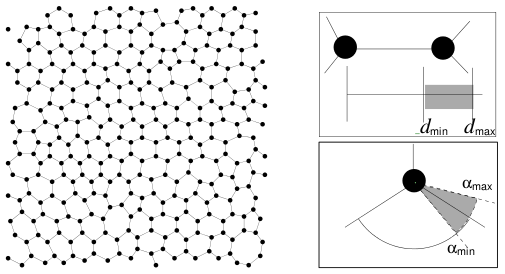
\includegraphics[width=10cm,height=5cm]{Figures/amorphousSilicon.png}
\label{fig:amorphousSilicon}
\end{figure}

\subsection{Simulated Annealing}
Simulated annealing is a stochastic approach towards minimizing an energy function.

\subsection{Genetic Algorithms}
Unlike simulated annealing, genetic algorithms rely on a population approach to 

\subsection{Ant-Colony Approaches}

\subsection{Go with the Winner Approaches}
Simulated annealing probabilistically convergences to the optimal solution at the rate
 of $O(\frac{1}{n})$ where n is the number of independent runs.  
Using heuristic schemes such as the ``Go with the Winner''~\cite{Aldous1994gwt}, hereby referred to as GWW, 
one can improve this convergence rate to $O(log \frac{1}{n})$ and have recently found their way into molecular modeling applications~\cite{Peinado1997gwt}.  In general terms, the GWW algorithm mirrors that of simulated annealing; however, each independent run is periodically reassessed to determine if one is converging upon a losing solution.  Runs with 
no chance for success are immediately discarded while runs with the best chance of finding an optimal solution
are replicated; thus, GWW generates an ensemble of independent runs filled with  ``winners''.  

\subsection{Analysis}
To assess the performance of our optimization schemes, we would


\bibliographystyle{plain}
\bibliography{AtomicScaleProposal}
\end{document}
